\documentclass[11pt,a4paper]{article}

\usepackage[margin=2cm]{geometry}
\usepackage[T1]{fontenc}
\usepackage{lmodern}
\usepackage{graphicx}
\usepackage{booktabs}
\usepackage{tabularx}
\usepackage{enumitem}
\usepackage{xcolor}
\usepackage{fancyvrb}
\usepackage[hidelinks]{hyperref}

\setlist{nosep}
\graphicspath{{figures/}}

% Placeholder for anything still to be decided or written. Search for
% "\todo" before submitting: none may be left in the final PDF.
\newcommand{\todo}[1]{\textcolor{red}{[TODO: #1]}}

\title{The Living Map: Spatial Memory for Emergency Robots\\[2pt]
  \large TSYP14 Technical Challenge --- IEEE RAS $\times$ AESS Tunisia}
\author{\todo{team name and members}}
\date{}

\begin{document}
\maketitle

% One file per section, so each owner edits only their own file.
% Owner: Bacha
\section{Introduction}
\todo{chosen environment; chosen events: gas, fire, victim (dead or alive), beacon out of range}
      % Bacha
% Owner: Ahmed
\section{Process}
\todo{PEB, Writer deploys PEB, Executor; include diagram}
           % Ahmed
% Owner: Ahmed
\section{Gazebo Simulation}
\todo{GitHub link or submitted video}
        % Ahmed
% Owner: Kais
\section{Network}

\subsection{Topology}

The network has three tiers (Fig.~\ref{fig:topology}). Inside the
disconnected zone, beacons dropped by the Writers form an ESP-NOW broadcast
mesh, and every robot is a node of that mesh. At each entrance, a pair of
wired \emph{Paired Entry Beacons} (PEB) bridges the mesh to the outside.
Outside, the PEB reaches the Command Post over 4G. No robot ever talks to the
Command Post directly: every frame passes through a PEB pair.

\begin{figure}[h]
\centering
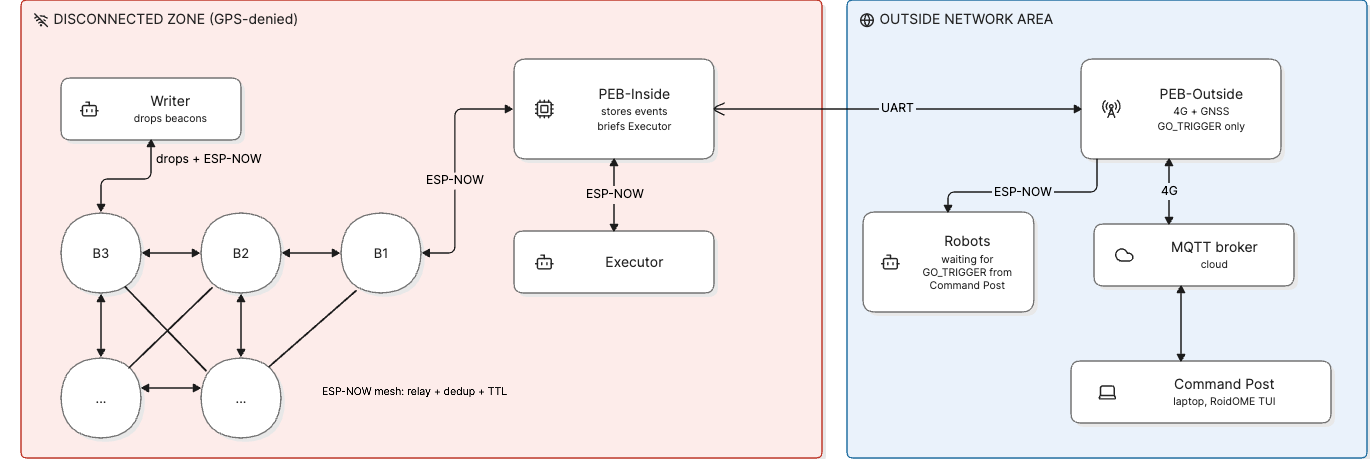
\includegraphics[width=\textwidth]{network-topology}
\caption{Network topology for one entrance.}
\label{fig:topology}
\end{figure}

\paragraph{Set-up.} Before any other task, and before taking instructions
from the Command Post, a Writer installs the infrastructure of its entrance:
PEB-Outside outside, PEB-Inside just past the entrance, joined by a
1--1.5\,m cable. Only then does it receive its GO\_TRIGGER and start exploring.

\paragraph{Data flow.} Events travel \emph{up}: Writer $\rightarrow$ beacon
mesh $\rightarrow$ PEB-Inside $\rightarrow$ cable $\rightarrow$ PEB-Outside
$\rightarrow$ 4G $\rightarrow$ Command Post. Orders travel \emph{down} the same
path. The operator chooses an Executor and sends a GO\_TRIGGER, which
PEB-Outside broadcasts over ESP-NOW to the robots waiting outside. The
briefing is split between the two halves because a briefing must happen at a
beacon: PEB-Outside only tells the Executor to \emph{enter}, and PEB-Inside
gives it the event details and its mission once it is inside.

\paragraph{Any number of robots and entrances.} Every robot has a unique
1-byte ID, so a GO\_TRIGGER can name its target Executor and every frame names
its Writer (Section~\ref{sec:message}). Each entrance has its own PEB pair. If
two meshes meet inside, a frame can leave through both pairs; the Command Post
keeps one copy per frame identifier.

\subsection{Network Communication: ESP-NOW}

All nodes inside the zone (beacons, PEBs, robots) use ESP-NOW, Espressif's
connectionless protocol on the 2.4\,GHz Wi-Fi radio:
\begin{itemize}
  \item \textbf{No infrastructure.} There is no access point, router or
    association; a node broadcasts and every node in range hears it. This
    suits a mesh whose nodes appear one by one as beacons are dropped, and
    disappear when they fail.
  \item \textbf{Fits our frames.} The 250-byte payload limit holds an event
    frame with up to 118 movement primitives ($14 + 2N$ bytes).
  \item \textbf{Low latency and low power.} A frame is sent in milliseconds,
    without a connection handshake.
  \item \textbf{One cheap chip.} The radio is built into the ESP8266/ESP32
    that each node needs anyway. Wi-Fi would need an access point, BLE has a
    shorter range, and LoRa needs an extra module and has a far lower data
    rate.
\end{itemize}
Beacons relay frames by flooding: a beacon drops a frame whose checksum is
wrong or whose \texttt{msg\_id} it has already seen, and decrements a hop
counter (TTL) before relaying. We validated relay, deduplication and TTL on a
bench of 3 ESP8266 nodes: every check passed with no send failure. Range has
not been measured yet. \todo{indoor range test}

\subsection{Paired Entry Beacons (PEB)}

The PEB is split into two halves, each built on the beacon hardware below with
its own battery, and joined by a cable carrying a UART link (TX, RX, GND,
115\,200\,baud). At 1--1.5\,m a plain UART is reliable; if the cable gets
longer or picks up motor noise, two RS-485 transceivers (about \$1 each) make
it robust over hundreds of metres. The same frames cross the cable as over the
air, each preceded by a start byte and a length byte.
\begin{itemize}
  \item \textbf{PEB-Inside} is a normal mesh beacon that also stores every
    event frame it receives, to brief Executors as they enter.
  \item \textbf{PEB-Outside} converts between the cable, ESP-NOW (to the
    robots waiting outside) and a 4G/LTE module with built-in GNSS
    \todo{module model}. The modem draws current peaks of about 2\,A, so it
    runs on a larger pack (2 $\times$ 18650).
\end{itemize}
PEB-Outside needs two serial ports, one for the cable and one for the modem.
The ESP8266 has only one full UART, so one link must use a software UART;
the ESP32 has three, which is one reason we plan to move to it.

\subsection{Beacons}

\begin{itemize}
  \item \textbf{Controller:} ESP8266 (ESP-NOW), moving to ESP32.
  \item \textbf{Power:} one 18650 Li-ion cell \todo{capacity}, its voltage
    read through a divider on the ADC.
  \item \textbf{Status LED:} off while the beacon is still carried by the
    Writer (not ready), steady on while broadcasting, blinking when the
    battery is low.
  \item \textbf{Enclosure:} 3D-printed (Section~\ref{sec:mechanics}).
\end{itemize}
A beacon keeps its frame in non-volatile memory, so it survives a reset, and
rebroadcasts it every 3\,s.

\subsection{Outside Network Area}

The Outside Network Area is made of PEB-Outside, a free cloud MQTT broker
and the Command Post. Over 4G, PEB-Outside sits behind the carrier's NAT and
cannot accept incoming connections, and neither can the Command Post laptop.
Both therefore connect \emph{out} to the broker:
\begin{itemize}
  \item PEB-Outside publishes incoming frames and its GNSS fix, and
    subscribes to GO\_TRIGGERs.
  \item The Command Post does the reverse.
\end{itemize}
Each entrance has its own topic (\texttt{livingmap/<entrance>/up},
\texttt{/down}, \texttt{/gps}), so adding an entrance needs no change at the
Command Post. The GNSS fix anchors the map of each entrance to real-world
coordinates (Section~\ref{sec:frame-translation}). The Command Post is a
laptop running our fork of the RoidOME terminal monitor, which already decodes
our frames live; reading from MQTT instead of a serial bridge is planned
for the next phase.
           % Kais
% Owner: Kais
\section{Message}\label{sec:message}

A beacon message must say \emph{what} was found, \emph{where} to go and
\emph{when} it was written, in a frame small enough for one ESP-NOW packet
(250 bytes). Fields are big-endian, and every frame ends with a checksum, the
XOR of all preceding bytes.

\paragraph{Identifier.} Every node that writes frames has a unique 1-byte
ID: \texttt{0x00} for the Command Post, \texttt{0x01}--\texttt{0x7F} for
Writers, \texttt{0x80}--\texttt{0xFE} for Executors. A frame is identified by
(frame type, \texttt{origin\_id}, \texttt{msg\_id}), where \texttt{msg\_id} is
a counter unique per origin. This tells which Writer composed each message,
and supports any number of robots. A beacon has no ID of its own: it is named
by the identifier of the frame it stores.

\paragraph{Event frame.} A Writer composes an EVENT\_BEACON frame and stores
it in the beacon it drops (Table~\ref{tab:event-frame}). It is $14 + 2N$
bytes long, where $N$ is the number of movement primitives (at most 118).

\begin{table}[h]
\centering
\small
\begin{tabularx}{\textwidth}{@{}l l l X@{}}
\toprule
Byte & Field & Size & Content \\
\midrule
0 & frame\_type & 1 & \texttt{0x01} \\
1 & origin\_id & 1 & Writer that composed it \\
2--3 & msg\_id & 2 & counter, unique per Writer \\
4 & ttl & 1 & hops left; decremented by each relay \\
5 & seq\_num & 1 & drop order in this Writer's run \\
6--9 & timestamp & 4 & seconds since this Writer's GO\_TRIGGER \\
10 & event\_type & 1 & \texttt{0x00} none (connectivity beacon), \texttt{0x01}
  gas, \texttt{0x02} fire, \texttt{0x03} victim alive, \texttt{0x04} victim
  dead, \texttt{0x05} robot down \\
11 & event\_value & 1 & severity, 0--255 \\
12 & primitive\_count & 1 & $N$ \\
13.. & primitives & $2N$ & path from the previous beacon: FORWARD (cm) or
  TURN (signed degrees) \\
last & checksum & 1 & XOR of all preceding bytes \\
\bottomrule
\end{tabularx}
\caption{EVENT\_BEACON frame.}
\label{tab:event-frame}
\end{table}

\paragraph{Where.} The primitives describe the path from the Writer's
previous beacon (from PEB-Inside for the first one). An Executor reaches an
event by following the beacons in drop order, and the Command Post rebuilds
every position by chaining these paths back to the entrance. Relative paths
keep frames short: their size depends on the distance between two beacons,
not on the distance from the entrance.

\paragraph{When, and message aging.} Messages age in three ways:
\begin{itemize}
  \item \textbf{Event age.} The timestamp counts seconds from the Writer's
    GO\_TRIGGER. The Command Post knows when it sent that order, so it turns
    every timestamp into real time and shows on the map how old each event is.
  \item \textbf{Hop limit.} Each relay decrements \texttt{ttl}, and a frame
    reaching 0 is no longer relayed, so no frame circulates forever.
  \item \textbf{Forgetting.} A beacon drops a frame it has already seen, but
    forgets it after 60\,s. Each frame is thus re-flooded about once a minute,
    and a node that arrives later, such as an Executor, still receives it.
\end{itemize}

\paragraph{Other frames.} Both start with the same first 5 bytes (type,
origin, \texttt{msg\_id}, \texttt{ttl}) and end with a checksum:
\begin{itemize}
  \item \textbf{GO\_TRIGGER} (8 bytes), from the Command Post: a
    \texttt{target\_id} (one robot, or all) and a \texttt{mission\_code}:
    explore or repair for a Writer, or the event type a robot must solve. Once the
    Executor is inside, PEB-Inside briefs it by replaying the stored event
    frames of that type, in drop order.
  \item \textbf{STATUS\_UPDATE} (8 bytes), from a beacon or a robot about
    itself: a status code (beacon low battery, or robot heartbeat) and its
    battery level (Section~\ref{sec:failure-cases}).
\end{itemize}
           % Kais
% Owners: Bacha (tank approach, 2FW drive), Hachicha (navigation, BMS and battery)
\section{Robot Hardware}
\todo{components of each robot}
   % Bacha, Hachicha
% Owners: Hachicha (writer navigation, executor entry and navigation), Bacha (event detection, executor types, mission decision)
\section{Navigation}
\subsection{Writer}
\todo{navigation (LiDAR, ...) --- Hachicha}

\todo{event detection (hardware, types) --- Bacha}
\subsection{Executor}
\todo{types of executors and how each solves an event --- Bacha}

\todo{mission decision --- Bacha}

\todo{entry and navigation: follows beacon drop order, and why --- Hachicha}
        % Hachicha, Bacha
% Owner: Bacha
\section{Frame Translation}\label{sec:frame-translation}
\todo{coordinate system (encoders and SLAM), origin at the PEB, math}
 % Bacha
% Owner: Kais
\section{Beacon Deposition Decision}

Beacons do two jobs: they mark where an event is, and they keep the chain of
radio links back to the PEB unbroken, so that every event reaches the Command
Post and an Executor can follow the chain. The Writer therefore drops a
beacon in two cases.

\paragraph{1. An event is detected.} The Writer stops at the event and drops
an \emph{event beacon} there (gas, fire, victim alive or dead), with the
severity and the path from its previous beacon. The beacon sits at the spot
the Executor must reach, so the last primitive of the path leads it exactly
there.

\paragraph{2. The Writer is about to lose the mesh.} The Writer runs an
ESP32, whose ESP-NOW receive callback reports the signal strength (RSSI) of
every frame. While exploring, it keeps hearing the 3\,s rebroadcasts of the
beacons behind it. When the strongest of them falls below a threshold
(about $-80$\,dBm \todo{calibrate}), it drops a \emph{connectivity beacon}
(event type \texttt{0x00}). The threshold sits above the level where ESP-NOW
stops working (around $-90$\,dBm), so the new beacon still has a reliable
link to the previous one. This uses beacons only where the building actually
weakens the signal (walls, corners, long corridors), instead of at a fixed
spacing that would waste them in open areas.

\paragraph{Loading and dropping.} Before a drop, the Writer sends the frame
by ESP-NOW unicast to the next beacon in its magazine. The beacon stores it
in non-volatile memory, turns its LED on and starts broadcasting; the
mechanism then releases it (Section~\ref{sec:mechanics}). The Writer moves on
without waiting for a confirmation; a beacon that fails is detected later by
the Command Post (Section~\ref{sec:failure-cases}).

\paragraph{Beacon budget.} A Writer carries $K$ beacons \todo{K, set by the
magazine}. When only 2 remain, it keeps them for events, stops exploring new
branches, and returns to the PEB to reload.
 % Kais
% Owner: Bacha
\section{Mechanics}\label{sec:mechanics}
\subsection{Tank Mechanical Design}
\todo{}
\subsection{Beacon Deposition Mechanism}
\todo{}
         % Bacha
% Owner: Kais
\section{Failure Cases}\label{sec:failure-cases}

The system is designed so that no single failure loses what was learned:
every event is stored in a beacon inside the zone, in PEB-Inside, and at the
Command Post. Table~\ref{tab:failures} lists how each failure is detected and
repaired. Repairs use two missions of the GO\_TRIGGER: \emph{repair}, which
sends a Writer to replace beacons, and \emph{take over}, which sends a robot
of the same type to continue the work of a robot that is down. In both cases
PEB-Inside briefs the robot with the stored frames it needs.

\begin{table}[h]
\centering
\small
\begin{tabularx}{\textwidth}{@{}p{2.2cm} X X@{}}
\toprule
Failure & Detection & Solution \\
\midrule
Robot battery dies
  & Every robot broadcasts a heartbeat with its battery level every 10\,s.
    At a critical level, the robot stops and broadcasts a \emph{robot down}
    frame with its position (path from its last beacon).
  & The robot spends its remaining energy as a beacon, relaying mesh
    traffic. Its knowledge is already in the beacons it dropped. The Command
    Post sends another robot of the same type to take over: a Writer resumes
    exploring from where the first one stopped, an Executor's mission is
    reassigned. \\
\addlinespace
Beacon battery dies
  & The beacon measures its battery; when low, its LED blinks and it
    broadcasts a low-battery status.
  & The Command Post sends a Writer on a repair mission. It drops a new
    beacon next to the old one and loads it with an exact copy of the old
    frame (same identifier), so nothing changes for the map or the
    Executors. \\
\addlinespace
Beacon destroyed
  & Each beacon's frame reaches the Command Post about once a minute (60\,s
    re-flood). No copy for 3 minutes means the beacon is lost. If a whole
    branch goes silent, the broken link is its silent beacon closest to the
    entrance.
  & Repair mission as above, the frame copied from PEB-Inside's store. An
    Executor already on its way keeps going: its brief holds the paths
    between beacons, so it can cross the gap by dead reckoning. \\
\addlinespace
PEB destroyed
  & PEB-Outside holds an MQTT connection to the broker, which publishes its
    \emph{last will} message the moment it drops off: the Command Post is
    alerted at once.
  & A Writer installs a spare PEB pair, at the same or another entrance.
    No data is lost: the beacons keep rebroadcasting, so the new PEB-Inside
    rebuilds its store within about a minute. \\
\bottomrule
\end{tabularx}
\caption{Failure cases, how they are detected, and how they are solved.}
\label{tab:failures}
\end{table}
     % Kais
% Owner: Bacha
\section{Implementation Plan}
\todo{scrum, sprints (add LEDs for beacons)}
    % Bacha
% Owner: Ahmed
\section{Conclusion}
\todo{}
        % Ahmed

\end{document}
